\documentclass[12pt,a4paper]{article}

% =====================================================
% Paquetes
% =====================================================
\usepackage[utf8]{inputenc}
\usepackage[T1]{fontenc}
\usepackage[spanish,es-nodecimaldot]{babel}
\usepackage{lmodern}
\usepackage{geometry}
\usepackage{setspace}
\usepackage{graphicx}
\usepackage{booktabs}
\usepackage{array}
\usepackage{xcolor}
\usepackage{listings}
\usepackage{microtype}
\usepackage{hyperref}
\usepackage{enumitem}
\usepackage{booktabs}
\usepackage{array}
\usepackage{float}
\usepackage{longtable}
\usepackage{graphicx}
\usepackage{subcaption}

% =====================================================
% Configuración de página y estilo
% =====================================================
\geometry{top=2.5cm,bottom=2.5cm,left=3cm,right=3cm}
\onehalfspacing
\setlength{\parindent}{1.2em}
\setlength{\parskip}{0.35em}

\definecolor{azul}{RGB}{31,78,121}
\definecolor{grisclaro}{RGB}{245,247,250}

\hypersetup{
    colorlinks=true,
    linkcolor=azul,
    citecolor=azul,
    urlcolor=azul,
    pdftitle={Recocido Simulado para la resolución del problema del agente viajero},
    pdfauthor={Ramírez Juárez María Fernanda}
}

\lstset{
    basicstyle=\ttfamily\small,
    backgroundcolor=\color{grisclaro},
    frame=single,
    rulecolor=\color{black!15},
    columns=fullflexible,
    keepspaces=true,
    showstringspaces=false,
    breaklines=true,
    tabsize=2
}

\setlist[description]{style=nextline,leftmargin=0pt,labelindent=0pt,itemsep=0.6em}

% =====================================================
% Información del documento
% =====================================================
\title{\textbf{Recocido Simulado para la resolución del problema del agente viajero}}
\author{Ramírez Juárez María Fernanda}
\date{\today}

% =====================================================
% Documento
% =====================================================
\begin{document}

\maketitle

% =====================================================
% 1. INTRODUCCIÓN
% =====================================================
\section{Introducción}
\label{sec:introduccion}

El problema del agente viajero (\textit{Traveling Salesman Problem}, TSP) es uno de los problemas de optimización combinatoria más estudiados en ciencias de la computación, y pertenece a la clase de problemas NP-duros. No se conoce un algoritmo que lo resuelva de manera exacta en tiempo polinomial, y el espacio de soluciones crece factorialmente con el número de ciudades. Ante esta limitación, las heurísticas metaheurísticas ofrecen una alternativa práctica: en lugar de garantizar la solución óptima, buscan soluciones de buena calidad en un tiempo de cómputo razonable.

Una de las metaheurísticas más influyentes para este tipo de problemas es el \textit{Recocido Simulado} (\textit{Simulated Annealing}), propuesta por Kirkpatrick, Gelatt y Vecchi en 1983 \cite{kirkpatrick1983}. Su idea central consiste en emular el proceso metalúrgico de recocido, en el cual un material se calienta y luego se enfría lentamente para reducir sus defectos estructurales. De manera análoga, el algoritmo permite que la búsqueda acepte, de forma probabilística, soluciones peores que la actual, especialmente al inicio, cuando la ``temperatura'' es alta, con el fin de escapar de mínimos locales. Posteriormente, la aceptación se restringe conforme la temperatura disminuye.

En 1990, Dueck y Scheuer propusieron una variante de esta heurística conocida como \textit{Aceptación por Umbrales} (\textit{Threshold Accepting}) \cite{dueck1990}, generalmente considerada más sencilla de implementar. A diferencia del recocido simulado clásico, donde la aceptación de una solución peor depende de una probabilidad calculada a partir de la diferencia de costos y la temperatura actual, la aceptación por umbrales utiliza un criterio determinista: una solución vecina se acepta si su costo no excede al de la solución actual en más de un umbral $T$. Este umbral se reduce gradualmente a lo largo de la ejecución. Esta es la heurística implementada en el presente proyecto para resolver instancias del TSP sobre un conjunto de ciudades con conexiones reales entre ellas.

% =====================================================
% 2. DESARROLLO
% =====================================================
\section{Desarrollo}

\subsection{Estructura del proyecto}
\label{sec:estructura}

El proyecto está organizado siguiendo una separación de responsabilidades por capas, típica de aplicaciones escritas enGo, la lógica de acceso a datos, el modelo del problema, la heurística de optimización y la generación de reportes viven en paquetes independientes dentro de \texttt{internal/}, mientras que el punto de entrada del programa se limita a orquestar la ejecución.
La Figura~\ref{fig:arbol} muestra la organización de directorios y archivos del proyecto.

\begin{figure}[H]
    \centering
    \begin{minipage}{0.92\textwidth}
\begin{lstlisting}
.
|-- cmd/tsp
|   |-- main.go
|   |-- paralelo.go
|-- config.json
|-- data
|   |-- input-150.tsp
|   |-- input-40.tsp
|-- internal
|   |-- data
|   |   |-- cargador.go
|   |   |-- db.go
|   |-- model
|   |   |-- camino.go
|   |   |-- grafica.go
|   |-- reporte
|   |   |-- graficaGNU.go
|   |   |-- reporte.go
|   |-- rs
|       |-- configuracion.go
|       |-- enfriamiento.go
|       |-- paralelizado.go
|       |-- recocido.go
|       |-- solucion.go
|       |-- vecino.go
|-- tsp.sql
\end{lstlisting}
    \end{minipage}
    \caption{Estructura de directorios del proyecto.}
    \label{fig:arbol}
\end{figure}

La Tabla~\ref{tab:capas} resume el propósito de cada capa antes de describirlas con más detalle.

\begin{table}[H]
\centering
\small
\renewcommand{\arraystretch}{1.25}
\begin{tabular}{@{}>{\raggedright\arraybackslash}p{2.5cm} >{\ttfamily}p{3cm} p{7cm}@{}}
\toprule
\textbf{Capa} & \textbf{Paquete} & \textbf{Responsabilidad} \\
\midrule
Entrada & cmd/tsp & Orquesta la ejecución: lee argumentos, construye la gráfica, corre la heurística y genera los reportes. \\
Datos & internal/data & Lee el archivo \texttt{.tsp} de entrada y consulta la base de datos SQLite. \\
Modelo & internal/model & Representa el problema como una gráfica y calcula distancias, costos y factibilidad. \\
Heurística & internal/rs & Implementa la aceptación por umbrales: solución inicial, vecindad, enfriamiento y búsqueda local. \\
Reportes & internal/reporte & Serializa los resultados de cada corrida y genera los datos para graficar la convergencia. \\
\bottomrule
\end{tabular}
\caption{Capas del proyecto y su responsabilidad principal.}
\label{tab:capas}
\end{table}

\subsection{Punto de entrada (\texttt{cmd/tsp})}

El archivo \texttt{main.go} recibe la ruta del archivo \texttt{.tsp} y los parámetros de configuración (\texttt{config.json}), construye la gráfica del problema a partir de la base de datos y ejecuta la heurística para una sola semilla o, mediante la bandera \texttt{-multi}, para varias semillas a la vez (\texttt{paralelo.go}), reportando en ambos casos el costo, la factibilidad y la trayectoria obtenida.

\subsection{Capa de datos (\texttt{internal/data})}

\begin{description}
  \item[\texttt{cargador.go}] Contiene \texttt{CargarArchivo}, que parsea el archivo de entrada \texttt{.tsp} y regresa la lista de identificadores de ciudad a considerar, y \texttt{RecibirArchivo}, que envuelve esta lectura para su uso desde el punto de entrada.
  \item[\texttt{db.go}] Contiene \texttt{GetCiudades}, que consulta la base de datos SQLite (\texttt{tsp.sql}) para obtener el nombre y las coordenadas geográficas de las ciudades solicitadas, junto con un mapa que traduce el identificador de cada ciudad a su posición dentro de las estructuras internas del programa.
\end{description}

\subsection{Capa de modelo (\texttt{internal/model})}

Esta capa define el tipo \texttt{GraficaTSP}, que representa la instancia del problema mediante una matriz de adyacencias (distancias reales entre ciudades) y los metadatos necesarios para trabajar con ella.

\begin{description}
  \item[\texttt{grafica.go}] Construye la gráfica (\texttt{ConstruirMatrizAdyacencias}): inicializa la matriz, carga las conexiones reales entre ciudades consultando la base de datos (\texttt{cargarConexiones}) y calcula la distancia geográfica entre dos puntos a partir de su latitud y longitud (\texttt{DistanciaNatural}, fórmula de Haversine). También incluye \texttt{CompletarAristas}, que sustituye las conexiones inexistentes por un peso penalizado en vez de dejarlas como infinitas, de modo que la heurística pueda operar incluso sobre gráficas dispersas, así como utilidades para copiar la gráfica o su matriz.
  \item[\texttt{camino.go}] Contiene las funciones para evaluar una trayectoria: \texttt{EvaluarTrayectoria} suma el costo (real o penalizado) de cada arista recorrida; \texttt{Costo} normaliza ese valor dividiéndolo entre \texttt{Normalizador}, la suma de las $n-1$ aristas más pesadas de la gráfica, usada como referencia de escala; \texttt{PesoAumentado} calcula el peso penalizado de una arista inexistente; y \texttt{EsFactible} determina si una trayectoria utiliza únicamente conexiones reales, a partir de la matriz original de la gráfica (antes de ser completada).
\end{description}

\subsection{Capa de heurística (\texttt{internal/rs})}

Esta es la capa central del proyecto, donde se implementa la aceptación por umbrales descrita en la Sección~\ref{sec:introduccion}.

\begin{description}
  \item[\texttt{configuracion.go}] Define el tipo \texttt{Parametros} (tamaño de lote, factor de enfriamiento, porcentaje de aceptación objetivo, entre otros) y \texttt{LeerParametros}, que los carga desde un archivo JSON.
  \item[\texttt{solucion.go}] Construye la solución inicial, ya sea como una permutación aleatoria de las ciudades (\texttt{SolucionInicial}) o mediante la heurística golosa de vecino más cercano (\texttt{SolucionInicialVecinoCercano}), que en la práctica ofrece un punto de partida de mejor calidad para la búsqueda.
  \item[\texttt{vecino.go}] Implementa \texttt{Vecino}, el operador de vecindad basado en \textit{2-opt}: invierte un segmento aleatorio de la trayectoria para generar una solución candidata.
  \item[\texttt{enfriamiento.go}] Calcula la temperatura inicial (\texttt{TemperaturaInicial}) mediante una búsqueda binaria (\texttt{BusquedaBinaria}) que ajusta el umbral hasta que el porcentaje de vecinos aceptados se acerque al valor objetivo definido en los parámetros. También contiene el ciclo principal de la heurística (\texttt{AceptacionPorUmbrales}), que reduce gradualmente el umbral y conserva la mejor solución encontrada.
  \item[\texttt{recocido.go}] Contiene \texttt{CalculaLote}, que agrupa un número fijo de soluciones aceptadas para estimar el costo promedio a una temperatura dada; \texttt{PorcentajeAceptados}, usado tanto en el cálculo de la temperatura inicial como en el diagnóstico de la búsqueda; \texttt{ResolverTSP}, que integra todo el proceso (construcción de la solución inicial, cálculo de la temperatura inicial, ciclo de enfriamiento y búsqueda local final); y \texttt{BusquedaLocal}, un barrido exhaustivo de \textit{2-opt} aplicado al final de la corrida para garantizar que la solución entregada sea un óptimo local respecto a esa vecindad, ya que durante la búsqueda principal se aceptan soluciones peores a propósito y no se garantiza haber probado todos los vecinos de la mejor solución encontrada.
  \item[\texttt{paralelizado.go}] Permite ejecutar \texttt{ResolverTSP} para varias semillas de forma simultánea (\texttt{ResolverTspParalelo}) y seleccionar la de menor costo entre las corridas exitosas (\texttt{MejorCorrida}).
\end{description}

\subsection{Capa de reportes (\texttt{internal/reporte})}

\begin{description}
  \item[\texttt{reporte.go}] Define las estructuras del reporte de ejecución y las funciones para guardarlo en formato JSON (\texttt{Guardar}) y como texto plano legible (\texttt{GuardarTXT}), incluyendo los parámetros usados, el costo, la factibilidad y la trayectoria de cada semilla.
  \item[\texttt{graficaGNU.go}] Genera, a partir del historial de convergencia de cada corrida, un archivo de datos y un \textit{script} de \texttt{gnuplot} (\texttt{GuardarConvergenciaGnuplot}) para graficar el costo de la mejor solución encontrada en función del número de evaluaciones realizadas.
\end{description}

\section{Resultados}
En esta sección se presentan los resultados obtenidos a partir de las corridas experimentales del algoritmo para dos casos de estudio: instancias de 40 y 150 ciudades. Entre los elementos evaluados destacan el costo de las soluciones, su factibilidad, el comportamiento de la convergencia y la comparación entre diferentes semillas.

Para evaluar el desempeño de la heurística, se realizaron diversas pruebas variando los parámetros de configuración, pero manteniendo las mismas semillas.

Las configuraciones utilizadas se muestran en la Tabla~\ref{tab:parametros}.

\begin{table}[H]
    \centering
    \caption{Configuraciones utilizadas en las pruebas para 40 y 150 ciudades.}
    \label{tab:parametros}
    \begin{tabular}{rrrrrrrr}
        \toprule
       Configuración & Lote & Máx. intentos & Máx. lotes & $\phi$ &
        $\epsilon$ & Aceptación & Iteraciones \\
        \midrule
      1 & 700 & 5000 & 200 & 0.996 & $10^{-6}$ & 0.90 & 200 \\
      2 & 30  & 500  & 50  & 0.85  & $10^{-6}$ & 0.90 & 50  \\
      3 & 150 & 8000 & 300 & 0.995 & $10^{-7}$ & 0.90 & 200 \\
      4 & 150 & 60   & 200 & 0.95  & $10^{-6}$ & 0.90 & 200 \\
      5 & 150 & 5000 & 2   & 0.95  & $10^{-6}$ & 0.90 & 200 \\
      6 & 1   & 5000 & 200 & 0.95  & $10^{-6}$ & 0.90 & 200 \\
        \bottomrule
    \end{tabular}
\end{table}

Primero analizaremos que suecede con 40 ciudades, para cada configuración se seleccionó la corrida que obtuvo el menor costo de trayectoria entre las semillas evaluadas. De esta manera, la comparación se centra en la calidad de la mejor solución encontrada bajo cada configuración.

Los resultados obtenidos se presentan en la Tabla~\ref{tab:resultados}.

\begin{table}[H]
    \centering
    \caption{Mejores resultados obtenidos para cada configuración.}
    \label{tab:resultados}
    \begin{tabular}{rrrr}
        \toprule
        Configuración & Semilla & Costo  $  Factibilidad  \\
        \midrule
        1 & 456 & 0.266356139166 & Sí \\
        2 & 1 & 0.270658188929 & Sí \\
        3 & 1 & 0.263819525597 & Sí \\
        4 & 789 & 0.273023506762 & Sí \\
        5 & 12345 & 0.266691569925 & Sí \\
        6 & 42 & 0.266691569925 & Sí \\
        \bottomrule
    \end{tabular}
\end{table}

En todos los casos se obtuvo una solución factible, lo que indica que las trayectorias seleccionadas cumplen con las restricciones de conectividad consideradas por el problema.\\
En términos del costo, se observa que existe una diferencia relativamente pequeña entre las configuraciones. El menor costo registrado corresponde a la configuración 3, con un valor de $0.263819525597$, mientras que el mayor corresponde a la configuración 4, con un valor de $0.273023506762$. Las configuraciones restantes presentan valores comprendidos entre estos dos extremos.

La diferencia absoluta entre el mejor y el peor resultado es:
[ 0.273023506762-0.263819525597=0.009203981165.]

Considerando el mejor resultado como referencia, esta diferencia representa aproximadamente un $3.49\%$. Por lo tanto, aunque existe una diferencia entre las configuraciones, los resultados se encuentran dentro de un intervalo relativamente reducido. Esto indica que, para la instancia de 40 ciudades, las modificaciones realizadas en los parámetros no producen cambios extremadamente grandes en el costo de la mejor solución encontrada.

La configuración 3 obtuvo el menor costo. Esta configuración utiliza un lote de 150 soluciones, un máximo de 8000 intentos por lote, hasta 300 lotes por temperatura, $\phi=0.995$ y $\epsilon=10^{-7}$. En comparación, la configuración 4 utiliza también un lote de 150, pero limita los intentos por lote a 60, utiliza $\phi=0.95$ y mantiene $\epsilon=10^{-6}$. La diferencia entre ambas configuraciones permite observar que el comportamiento de la heurística no depende de un único parámetro, sino de la combinación de tamaño de lote, número de intentos y estrategia de enfriamiento.

Por otro lado, la configuración 4 obtuvo el costo más alto entre las seis configuraciones. Su comportamiento puede estar relacionado con la combinación de un valor de $\phi$ menor y un número considerablemente menor de intentos por lote. Un valor menor de $\phi$ provoca una reducción más rápida de la temperatura, mientras que el límite de 60 intentos restringe la cantidad de soluciones exploradas dentro de cada lote. Esto puede reducir el tiempo de búsqueda, aunque también puede limitar la exploración del espacio de soluciones.

Es importante señalar que la comparación presentada corresponde exclusivamente a las mejores corridas de cada configuración. Por ello, estos resultados permiten comparar la mejor solución encontrada, pero no describen por sí solos la variabilidad o estabilidad de cada configuración. Para realizar un análisis más completo sería conveniente considerar también el promedio, el peor resultado, la desviación entre semillas, el número de evaluaciones realizadas y el comportamiento de convergencia.

En cuanto a las semillas, se observa que las mejores soluciones no fueron obtenidas siempre con la misma semilla. Por ejemplo, la configuración 1 obtuvo su mejor resultado con la semilla 456, mientras que las configuraciones 2 y 3 lo obtuvieron con la semilla 1. Esto es consistente con el carácter estocástico de la heurística, ya que diferentes semillas generan diferentes secuencias de soluciones candidatas y, por lo tanto, pueden conducir a resultados distintos.

Ahora podemos pasar al analisis del comportamiento de nuestros datos:\\
Grafica de convergencia.
\begin{figure}[htbp]
    \centering
    \begin{subfigure}[b]{0.48\textwidth}
        \centering
        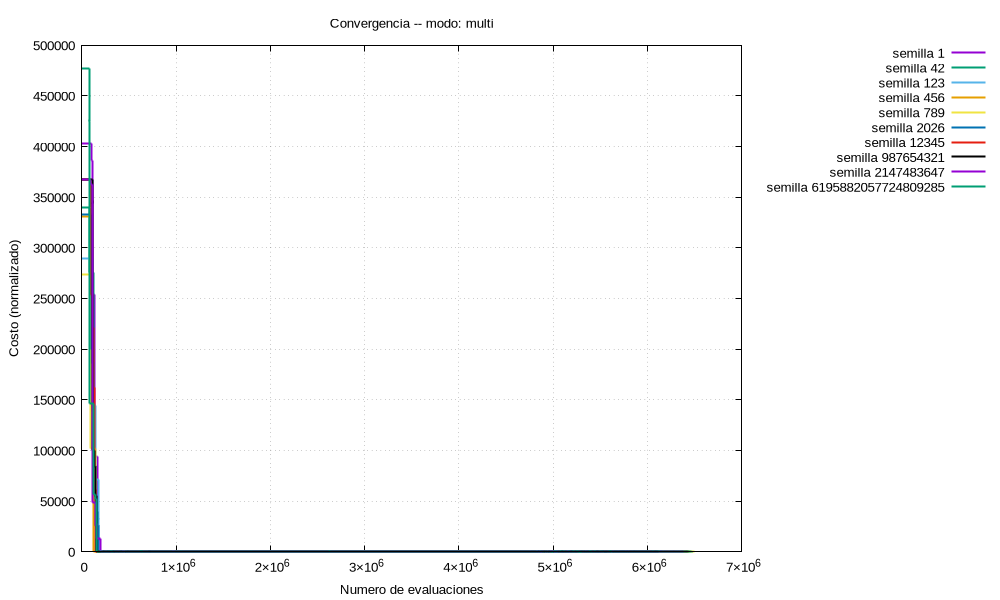
\includegraphics[width=\textwidth]{1.2.png}
        \caption{Mejor evaluación}
        \label{fig:imagen1}
    \end{subfigure}
    \hfill % Relleno horizontal entre las imágenes
    \begin{subfigure}[b]{0.48\textwidth}
        \centering
        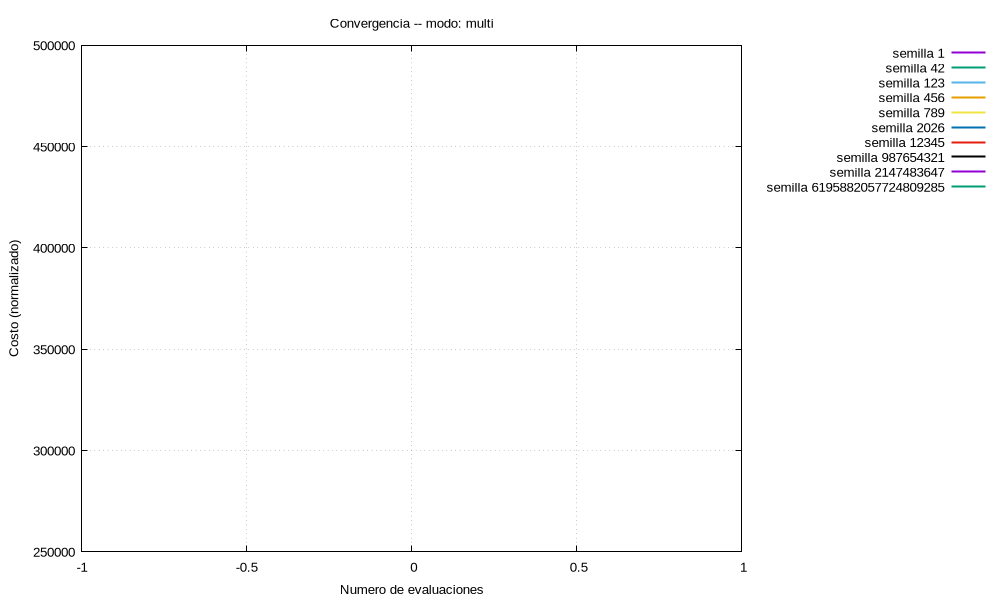
\includegraphics[width=\textwidth]{1.3.png}
        \caption{Peor evalución}
        \label{fig:imagen2}
    \end{subfigure}
\end{figure}

En la gráfica de convergencia correspondiente a la configuración con el mejor resultado se observa una disminución rápida del costo durante las primeras evaluaciones. Posteriormente, la curva alcanza una región prácticamente estable y permanece alrededor de este valor durante el resto de la ejecución. Este comportamiento indica que la mayor parte de la mejora de la solución se concentra en las etapas iniciales de la búsqueda, mientras que las evaluaciones posteriores producen cambios cada vez menores.

Para la configuración correspondiente al peor resultado no se obtuvo una curva visible en la gráfica de convergencia. Este comportamiento puede estar relacionado con la cantidad de información registrada durante la ejecución y con la configuración de los parámetros. En particular, esta configuración utiliza max\_intentos\_por\_lote = 60 y $\phi=0.95$, por lo que se realizan menos intentos por lote y la temperatura disminuye más rápidamente. Esto puede reducir la cantidad de evaluaciones registradas y limitar la duración de la exploración del espacio de soluciones.

Trayectorias:

\begin{quote}
  \textit{Configuración 3 (semilla 1):}\\[0.5em]
  \footnotesize
  $979, 493, 329, 163, 172, 496, 815, 657, 168, 1,656, 2, 653, 490, 654, 7, 816, 982, 332, 820, 981, 333,$\\
  $3, 165, 6, 5, 978, 817, 4, 489, 492, 491, 984, 331, 164, 327, 980, 244, 75, 652$
\end{quote}

 
\begin{quote}
  \textit{Configuración 4 (semilla 789):}\\[0.5em]
  \footnotesize
  $657, 168, 1, 7, 816, 982, 332, 820, 654, 490, 653, 2, 656, 815, 172, 496, 329, 163, 493, 979, 4, 165,$\\
  $3, 333, 981, 6, 5, 978, 817, 489, 492, 491, 984, 331, 164, 327, 980, 244, 75, 652$
\end{quote}

\begin{figure}[htbp]
    \centering
    \begin{subfigure}[b]{0.48\textwidth}
        \centering
        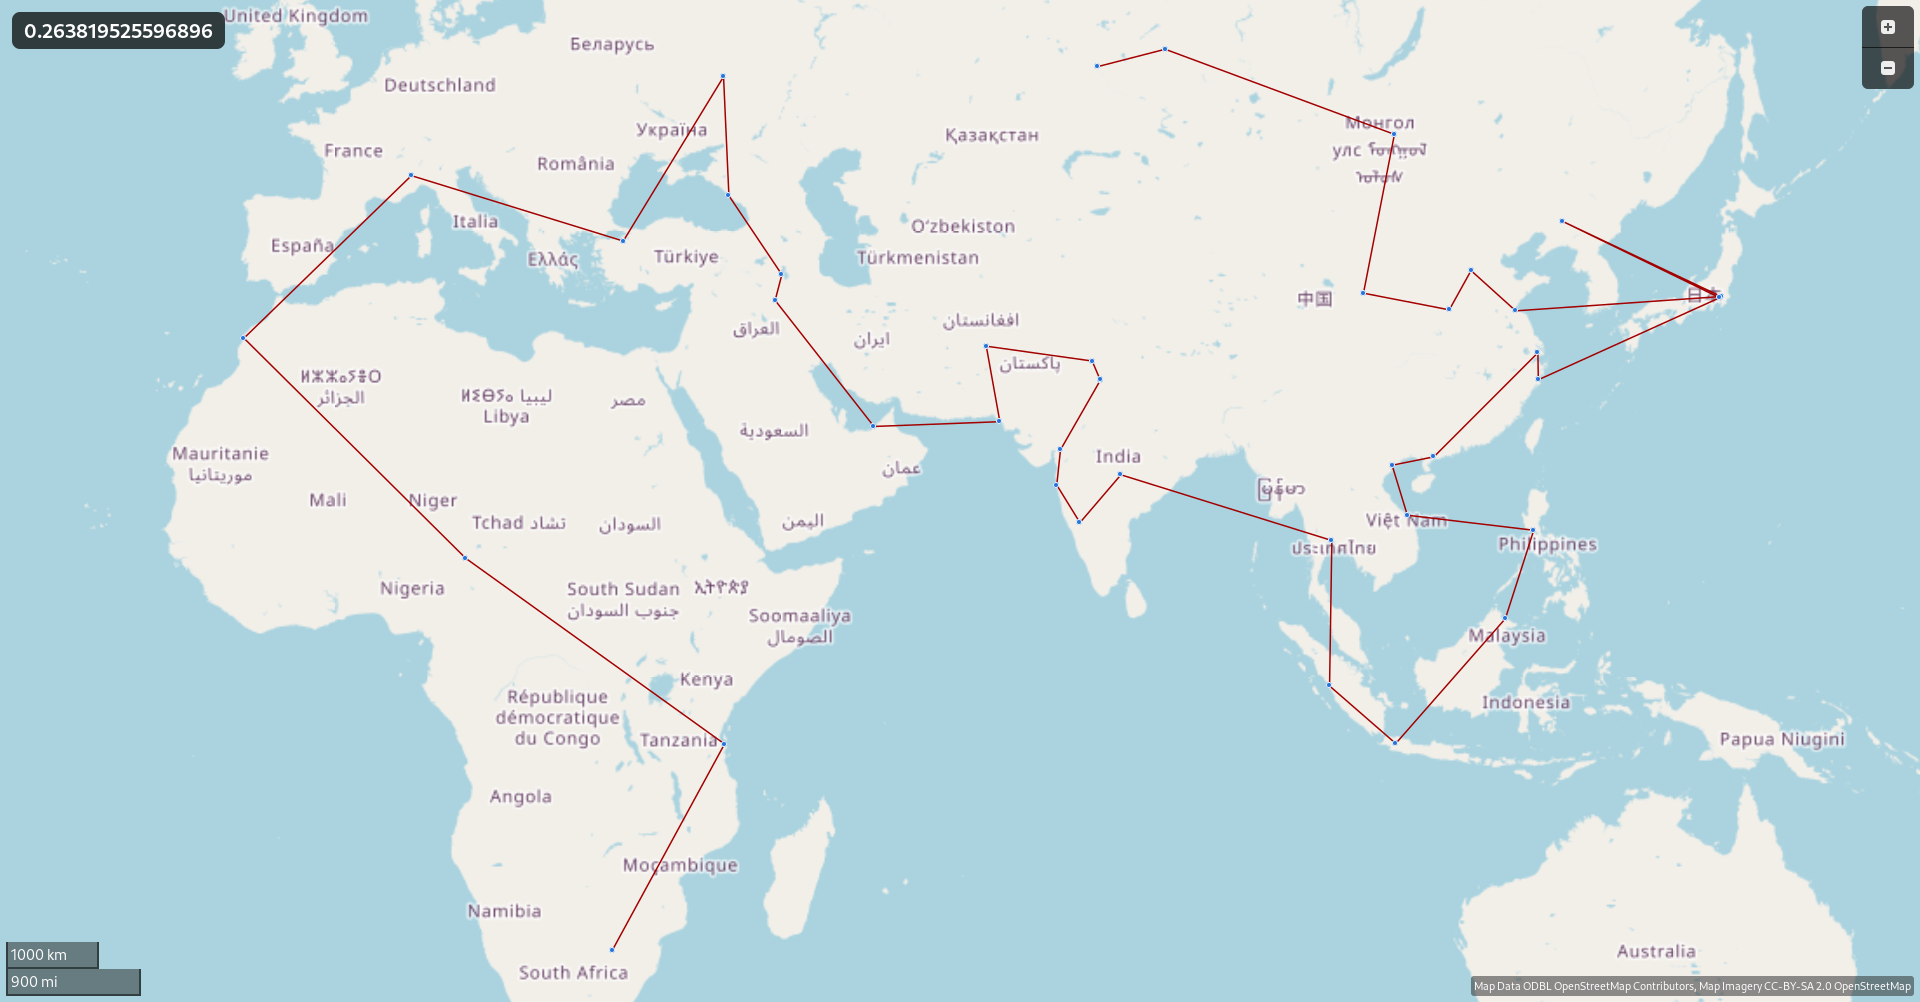
\includegraphics[width=\textwidth]{mapa-40-buena.png}
        \caption{Mejor evaluación}
        \label{fig:imagen1}
    \end{subfigure}
    \hfill % Relleno horizontal entre las imágenes
    \begin{subfigure}[b]{0.48\textwidth}
        \centering
        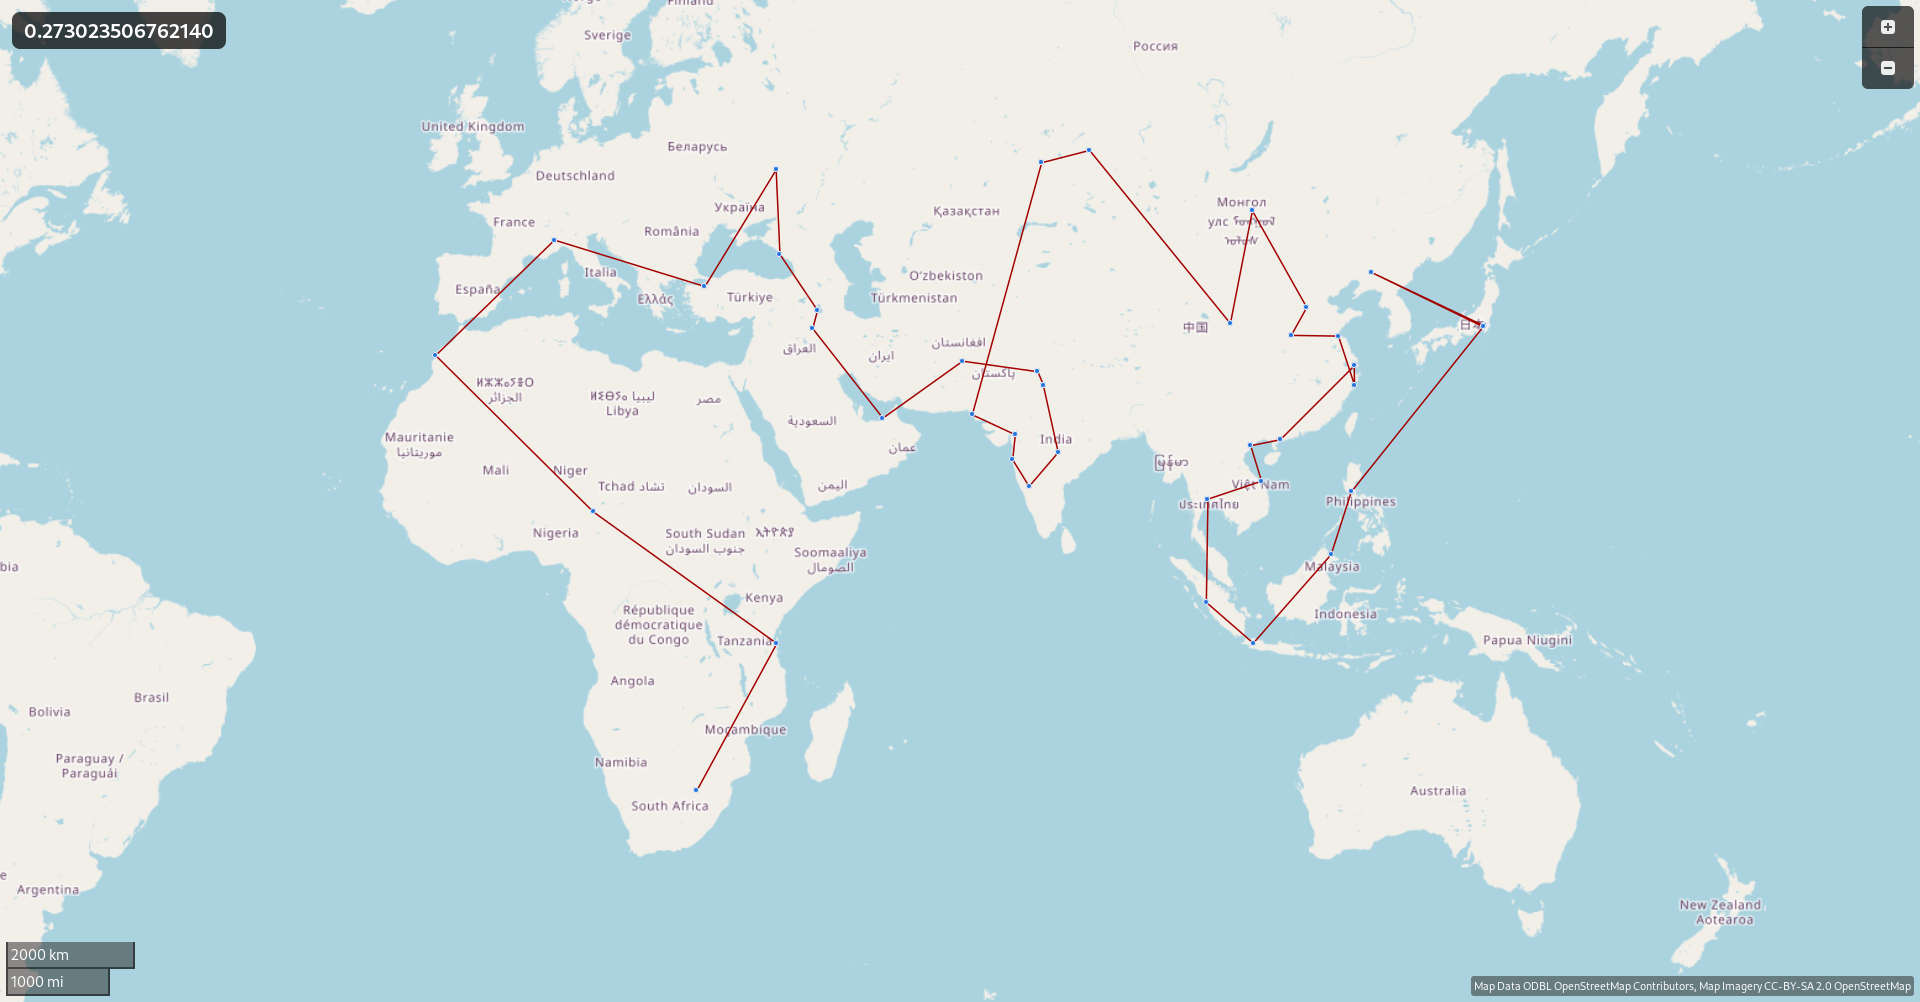
\includegraphics[width=\textwidth]{mapa-40-peor.png}
        \caption{Peor evalución}
        \label{fig:imagen2}
    \end{subfigure}
    \label{fig:dos_imagenes}
\end{figure}

Al comparar las trayectorias obtenidas para las configuraciones analizadas, se observa que presentan un recorrido espacial muy similar. Esto indica que, aunque los parámetros modifican el proceso de búsqueda, ambas ejecuciones pueden llegar a regiones cercanas del espacio de soluciones y construir recorridos con características similares.

Las diferencias entre las trayectorias pueden estar relacionadas con el carácter estocástico de la heurística y con los parámetros utilizados en cada configuración. En particular, el número de intentos por lote y la velocidad de enfriamiento influyen en la cantidad de soluciones candidatas exploradas y en la posibilidad de aceptar movimientos durante el proceso de búsqueda.


Para la instancia de 150 ciudades se realizaron las mismas seis configuraciones de parámetros, con el objetivo de analizar cómo se comporta la heurística al incrementar el tamaño del problema. La Tabla~\ref{tab} presenta el mejor resultado obtenido para cada configuración, considerando las diferentes semillas utilizadas.

\begin{table}[H]
    \centering
    \caption{Mejores resultados obtenidos para cada configuración.}
    \label{tab:resultados}
    \begin{tabular}{rrrr}
        \toprule
        Configuración & Semilla & Costo & Factibilidad  \\
        \midrule
        1 & 987654321, & 0.145611992266 & Sí \\
        2 & 42 & 0.141622492351 & Sí \\
        3 & 2147483647, & 0.140993722694 & Sí \\
        4 & 12345 & 41081.353411326883 & NO \\
        5 & 456 & 0.141436602455 & Sí \\
        6 & 123 & 0.148762498164 & Sí \\
        \bottomrule
    \end{tabular}
\end{table}

Se observa que cinco de las seis configuraciones obtuvieron una solución factible. Los costos de estas soluciones se encuentran en un intervalo relativamente reducido, desde $0.140993722694$ hasta $0.148762498164$. La configuración 3 obtuvo el menor costo registrado, con $0.140993722694$, utilizando la semilla $2147483647$.

Por otro lado, la configuración 4 presenta un comportamiento considerablemente diferente. Su mejor resultado registrado tiene un costo de $41081.353411326883$ y fue clasificado como no factible. Esta diferencia es muy grande respecto a los valores obtenidos por las demás configuraciones, por lo que no puede considerarse simplemente una variación pequeña del costo entre semillas o configuraciones.

Para simplificar el análisis detallado, se seleccionaron dos casos extremos dentro de los resultados obtenidos: la configuración 3, que presentó el menor costo, y la configuración 4, que presentó el mayor costo y además una solución no factible. La comparación se presenta en la Tabla~\ref{tab:comparación1}.

\begin{table}[H]
    \centering
    \caption{Comparartiva}
    \label{tab:comparación1}
    \begin{tabular}{rrrr}
        \toprule
        Configurción & Semilla & Resultado  \\
        \midrule
        3 & 2147483647 & 0.140993722694  \\
        4 & 12345 & 41081.353411326883 \\
        \bottomrule
    \end{tabular}
\end{table}

La configuración 3 utiliza un lote de 150 soluciones, hasta 8000 intentos por lote, un máximo de 300 lotes por temperatura, $\phi=0.995$ y $\epsilon=10^{-7}$. En contraste, la configuración 4 utiliza un lote de 150 soluciones, únicamente 60 intentos por lote, $\phi=0.95$ y $\epsilon=10^{-6}$. Por lo tanto, existen diferencias importantes en la cantidad de intentos permitidos y en la velocidad de enfriamiento.

El valor de $\phi=0.95$ utilizado por la configuración 4 provoca un enfriamiento más rápido que el valor de $\phi=0.995$ de la configuración 3. Además, el límite de 60 intentos por lote reduce considerablemente la cantidad de movimientos que pueden explorarse antes de modificar la temperatura. Esta combinación puede limitar la exploración del espacio de soluciones y favorecer que el algoritmo finalice sin encontrar una trayectoria factible de bajo costo.

En cambio, la configuración 3 permite realizar una búsqueda más prolongada debido al mayor número de intentos por lote y al enfriamiento más gradual. Esto proporciona más oportunidades para explorar distintas soluciones antes de que la temperatura alcance valores bajos. En esta instancia, dicho comportamiento se relaciona con la obtención de una solución factible con el menor costo registrado.

Sin embargo, estos resultados deben interpretarse con precaución. El hecho de que la configuración 3 haya obtenido el menor costo no significa, por sí solo, que sea la configuración óptima para cualquier instancia. Los resultados corresponden específicamente a la instancia de 150 ciudades, las semillas utilizadas y los parámetros establecidos para este experimento.

Un aspecto particularmente relevante es la diferencia de comportamiento entre las configuraciones 3 y 4. Mientras que la configuración 3 obtuvo una solución factible con un costo de $0.140993722694$, la configuración 4 terminó con una solución no factible y un valor de $41081.353411326883$. Esto sugiere que, para esta instancia, la combinación de parámetros utilizada en la configuración 4 puede resultar insuficiente para explorar adecuadamente el espacio de soluciones. No obstante, para determinar con mayor certeza la causa de este comportamiento es necesario analizar también las estadísticas de soluciones factibles y no factibles, el número de evaluaciones realizadas y las curvas de convergencia de ambas configuraciones.\\

Realizamos el análisis de la gráfica de convergencia.

\begin{figure}[htbp]
    \centering
    \begin{subfigure}[b]{0.48\textwidth}
        \centering
        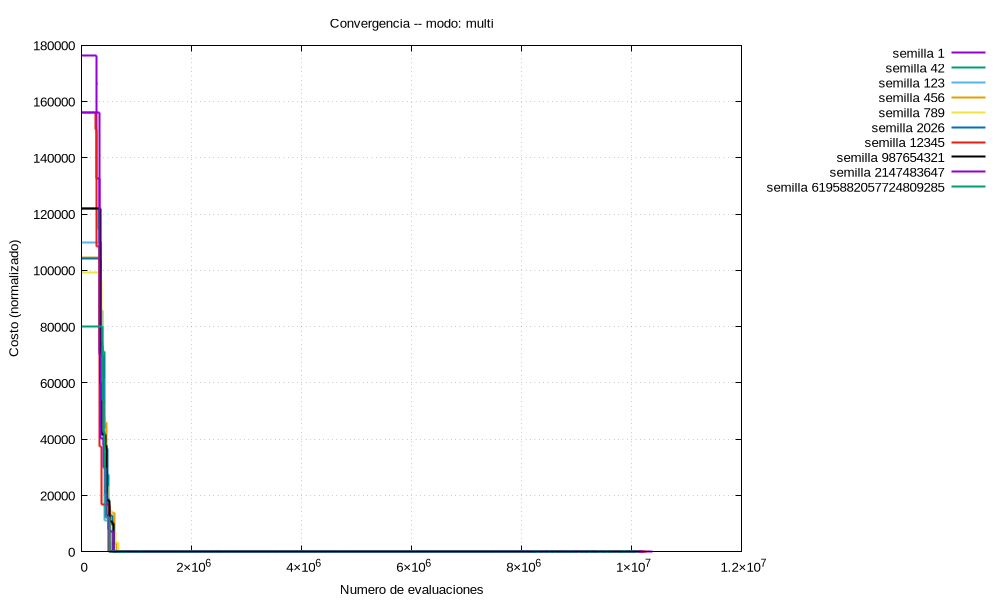
\includegraphics[width=\textwidth]{2.2.png}
        \caption{Mejor evaluación}
        \label{fig:imagen1}
    \end{subfigure}
    \hfill % Relleno horizontal entre las imágenes
    \begin{subfigure}[b]{0.48\textwidth}
        \centering
        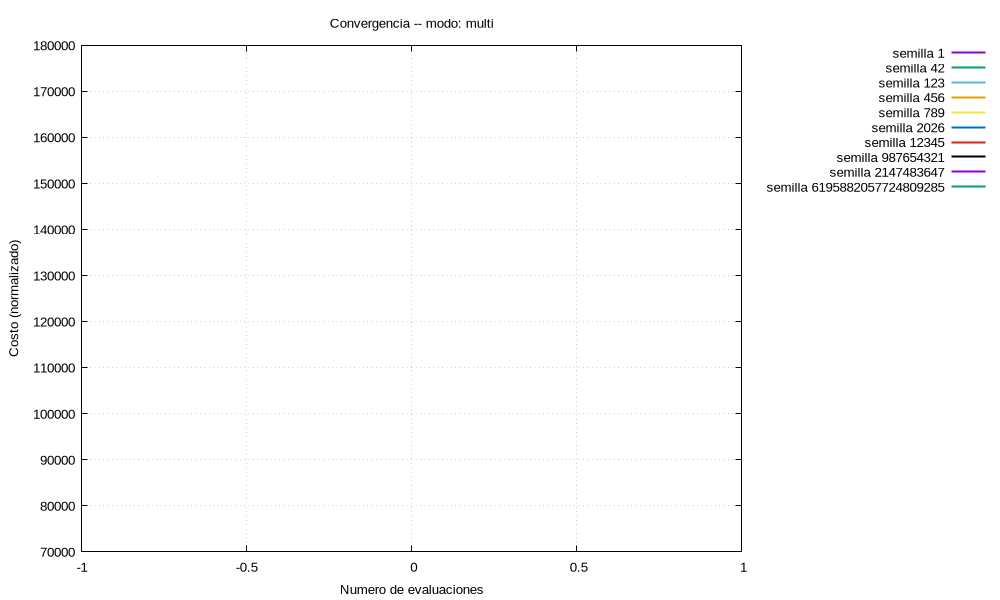
\includegraphics[width=\textwidth]{2.3.png}
        \caption{Peor evaluación}
        \label{fig:imagen2}
    \end{subfigure}
    \label{fig:dos_imagenes}
\end{figure}


El comportamiento observado en las gráficas de convergencia para la instancia de 150 ciudades es similar al presentado anteriormente para la instancia de 40 ciudades. En ambos casos, la mayor variación del costo se concentra durante las primeras etapas de la búsqueda, mientras que posteriormente la curva presenta una tendencia más estable.

Debido a que el comportamiento de las curvas es semejante al caso de 40 ciudades, no se considera necesario repetir el análisis detallado de la convergencia. Por ello, en esta sección se centra la atención en el análisis visual de las trayectorias obtenidas, particularmente en la diferencia entre la solución factible y la solución no factible.

Trayectorias:

\begin{quote}
  \textit{Configuración 3 (semilla 2147483647):}\\[0.5em]
  \footnotesize
  $183,75,346,77,171,652,1075,483,512,821,179,671,16,520,186,675,1038,12,828,502,$
  $340,244,339,826,444,17,25,492,491,499,347,817,489,4,174,23,176,668,352,978,5,6,$
  $988,165,3,981,333,990,353,27,991,185,22,351,1004,163,676,665,344,653,490,654,26,$
  $820,345,332,181,14,982,187,816,678,823,7,507,2,656,667,184,173,673,839,496,182,172,$
  $815,9,832,663,657,661,829,1,986,508,168,505,19,329,509,493,979,837,995,984,501,164,$
  $11,1003,349,331,662,8,999,334,674,985,343,510,660,20,825,500,504,511,327,670,350,840,$
  $336,980,297,1001,74,822,166,658,666,818,655,819,330,1073,169,1037,326,328,167,495,494$

\end{quote}

 
\begin{quote}
  \textit{Configuración 4 (semilla 12345):}\\[0.5em]
  \footnotesize
  $166,658,666,818,655,819,330,1073,169,1037,326,328,167,495,494,510,660,20,343,985,$
  $500,825,504,511,327,670,350,840,336,980,297,1001,74,822,828,12,1038,502,340,675,$
  $186,520,16,652,1075,483,171,77,183,346,75,821,512,179,671,339,244,826,444,17,501,$
  $164,11,1003,349,674,334,999,8,662,331,995,984,491,499,492,25,489,817,347,837,979,$
  $493,509,329,19,839,496,182,172,163,673,665,676,22,185,351,1004,6,5,978,352,668,176,$
  $23,988,174,4,165,3,981,990,353,27,333,991,26,820,345,332,181,14,982,187,816,678,823,$
  $7,654,490,344,653,507,2,656,667,184,173,815,505,168,9,832,661,663,657,829,1,986,508$


\end{quote}

\begin{figure}[htbp]
    \centering
    \begin{subfigure}[b]{0.48\textwidth}
        \centering
        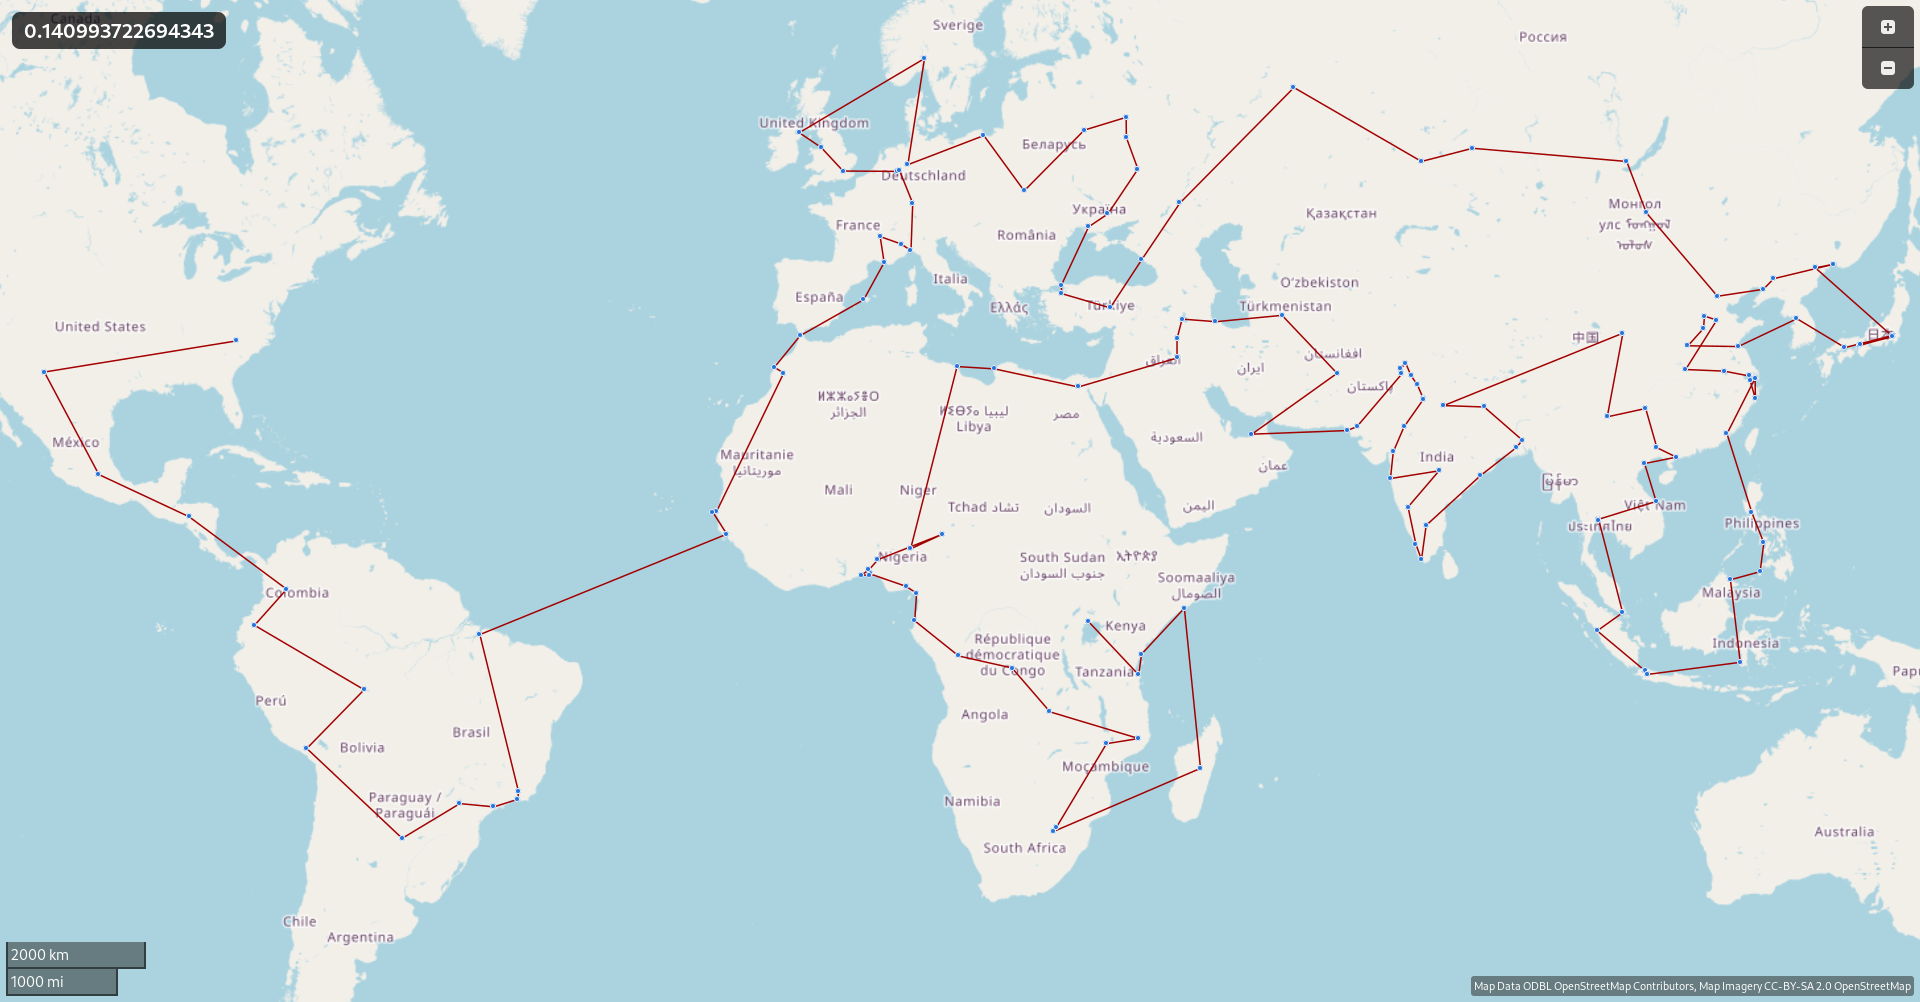
\includegraphics[width=\textwidth]{mapa-150-buena.png}
        \caption{Mejor evaluación}
        \label{fig:imagen1}
    \end{subfigure}
    \hfill % Relleno horizontal entre las imágenes
    \begin{subfigure}[b]{0.48\textwidth}
        \centering
        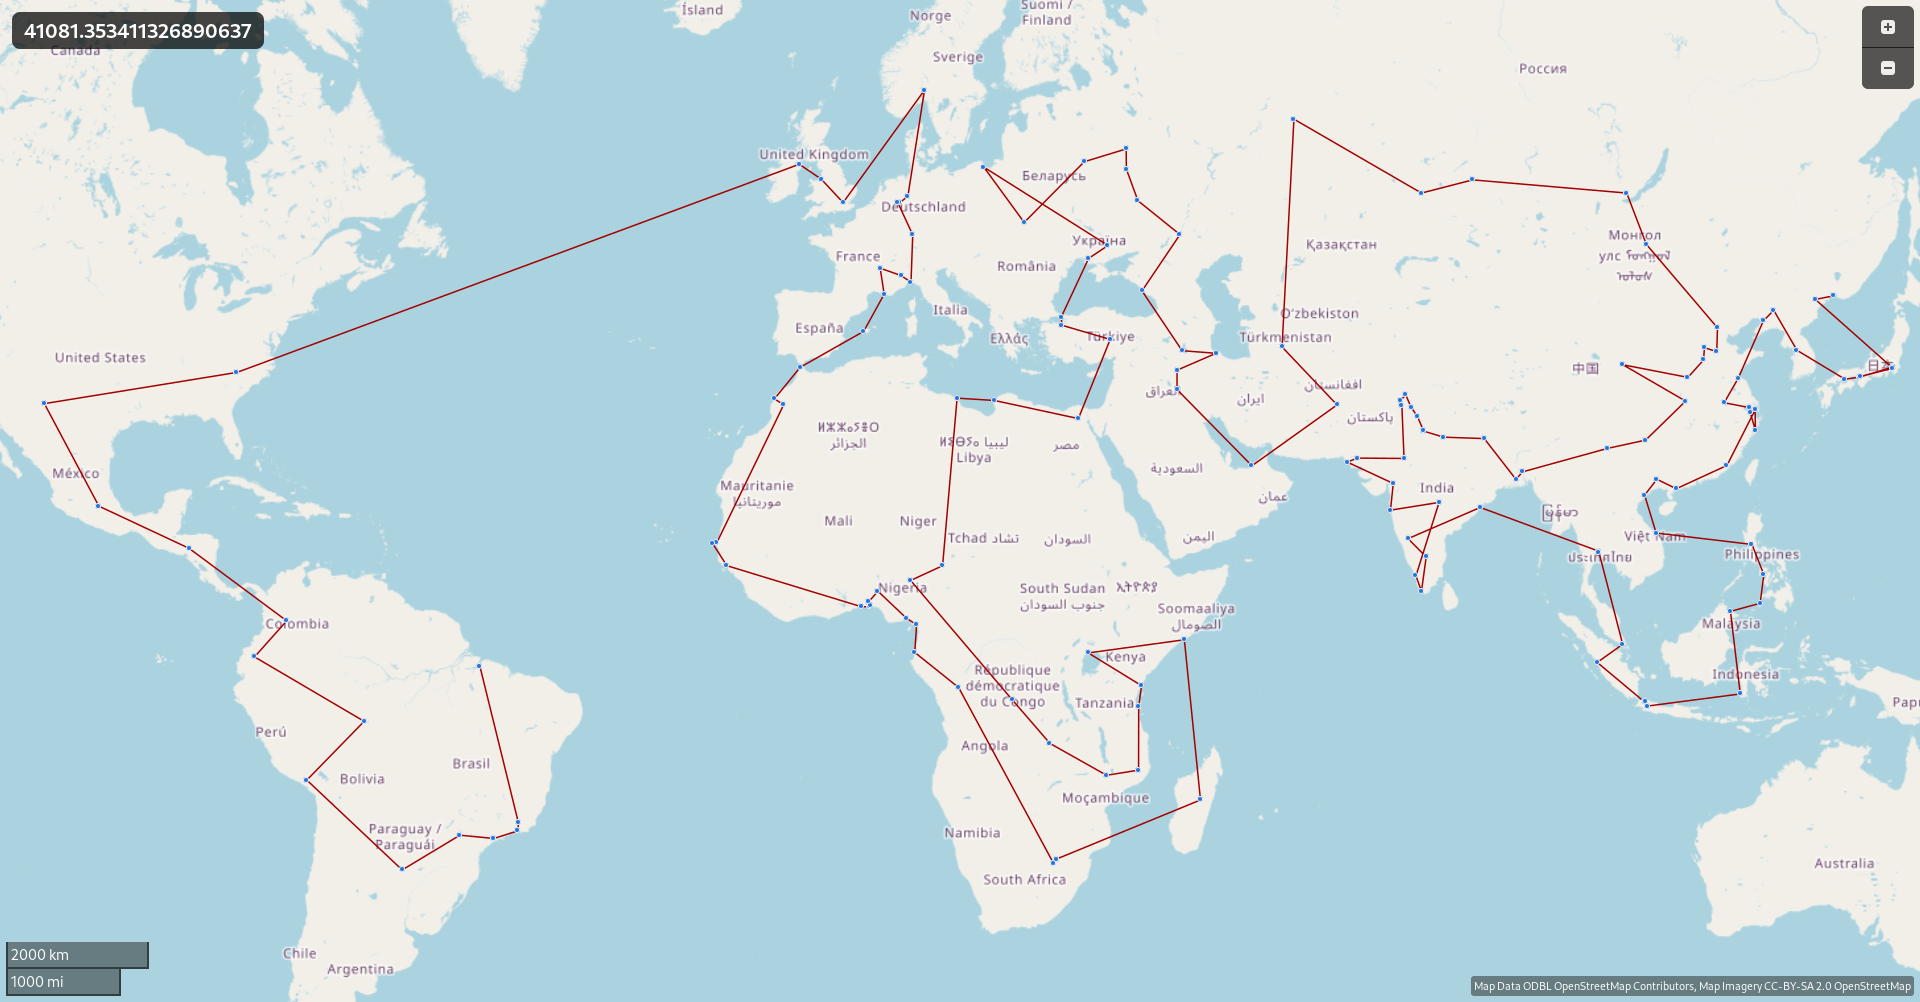
\includegraphics[width=\textwidth]{mapa-150-mala.png}
        \caption{Peor evalución}
        \label{fig:imagen2}
    \end{subfigure}
    \label{fig:dos_imagenes}
\end{figure}

En este caso, la diferencia entre ambas trayectorias resulta más evidente. En el mapa correspondiente a la configuración 4, cuya solución fue clasificada como no factible, se puede observar que la trayectoria utiliza al menos una conexión entre dos ciudades para las cuales no existe una arista en la instancia original. Esta conexión se identifica visualmente como un segmento que une dos ciudades que no cuentan con una conexión válida.

Este comportamiento es consistente con el resultado obtenido en la tabla, donde la configuración 4 presenta una solución no factible y un costo considerablemente mayor que el resto de las configuraciones. La utilización de una arista inexistente hace que la trayectoria no cumpla con las restricciones del problema y, además, contribuye al incremento del costo mediante la penalización utilizada por el algoritmo para representar las conexiones no disponibles.

Por el contrario, en el mapa correspondiente a la configuración 3 se observa una trayectoria factible. En este caso, las conexiones utilizadas corresponden a aristas existentes en la instancia, por lo que la trayectoria cumple con las restricciones de conectividad consideradas. Esto es consistente con su clasificación como solución factible y con el bajo costo obtenido de $0.140993722694$.

La comparación visual permite complementar los resultados numéricos de la tabla: mientras que la configuración 3 encuentra una trayectoria válida entre las ciudades, la configuración 4 termina utilizando conexiones no disponibles. Por lo tanto, el análisis de las trayectorias ayuda a identificar visualmente una de las posibles causas del comportamiento tan diferente entre ambas configuraciones.

% =====================================================
% 3. CONCLUSIÓN
% =====================================================
\section{Conclusión}

El proyecto permitió implementar una estrategia heurística basada en aceptación por umbrales para resolver el problema del agente viajero, combinando una solución inicial, una vecindad \textit{2-opt}, un esquema de enfriamiento progresivo y una búsqueda local final. La separación en capas facilitó la organización del sistema y el análisis de los resultados obtenidos.

En la instancia de 40 ciudades, todas las configuraciones evaluadas obtuvieron soluciones factibles y los costos presentaron diferencias relativamente pequeñas. El menor costo registrado fue de $0.263819525597$, correspondiente a la configuración 3, mientras que el mayor fue de $0.273023506762$, correspondiente a la configuración 4.

Para la instancia de 150 ciudades se observaron diferencias más marcadas entre las configuraciones. Cinco obtuvieron soluciones factibles con costos cercanos entre sí, mientras que la configuración 4 produjo una solución no factible con un costo de $41081.353411326883$. El análisis de su trayectoria permitió identificar el uso de conexiones que no existen en la instancia original, lo que explica su falta de factibilidad y el elevado costo obtenido.

Las gráficas de convergencia mostraron que la mayor reducción del costo ocurre durante las primeras etapas de la búsqueda y posteriormente se presenta una tendencia más estable. Además, las diferencias entre semillas y configuraciones muestran el carácter estocástico de la heurística y la importancia de analizar varias corridas.

En conjunto, los experimentos muestran que el comportamiento de la heurística depende tanto de los parámetros utilizados como del tamaño de la instancia, siendo necesario considerar conjuntamente el costo, la factibilidad y la convergencia para evaluar sus resultados.


% =====================================================
% 4. REFERENCIAS
% =====================================================
\begin{thebibliography}{99}

\bibitem{kirkpatrick1983}
Kirkpatrick, S., Gelatt, C. D., y Vecchi, M. P. (1983).
\textit{Optimization by Simulated Annealing}.
\textit{Science}, 220(4598), 671--680.

\bibitem{dueck1990}
Dueck, G., y Scheuer, T. (1990).
\textit{Threshold Accepting: A General Purpose Optimization Algorithm Appearing Superior to Simulated Annealing}.
\textit{Journal of Computational Physics}, 90(1), 161--175.

\end{thebibliography}

\end{document}
